\documentclass[%
a4paper,							% alle weiteren Papierformat einstellbar
%landscape,						% Querformat
12pt,								% Schriftgröße (12pt, 11pt (Standard))
%BCOR1cm,							% Bindekorrektur, bspw. 1 cm
%DIVcalc,							% führt die Satzspiegelberechnung neu aus
%											  s. scrguide 2.4
%twoside,							% Doppelseiten
%twocolumn,						% zweispaltiger Satz
%halfparskip*,				% Absatzformatierung s. scrguide 3.1
parskip=half,
%headsepline,					% Trennline zum Seitenkopf	
%footsepline,					% Trennline zum Seitenfuß
%titlepage,						% Titelei auf eigener Seite
%normalheadings,			% Überschriften etwas kleiner (smallheadings)
%idxtotoc,						% Index im Inhaltsverzeichnis
%liststotoc,					% Abb.- und Tab.verzeichnis im Inhalt
%bibtotoc,						% Literaturverzeichnis im Inhalt
%abstracton,					% Überschrift über der Zusammenfassung an	
%leqno,   						% Nummerierung von Gleichungen links
%fleqn,								% Ausgabe von Gleichungen linksbündig
%draft								% überlangen Zeilen in Ausgabe gekennzeichnet
]
{article}


%% Deutsche Anpassungen %%%%%%%%%%%%%%%%%%%%%%%%%%%%%%%%%%%%%
\usepackage[ngerman]{babel}
\usepackage[T1]{fontenc}
\usepackage[utf8]{inputenc}
\usepackage{lmodern} %Type1-Schriftart für nicht-englische Texte
\usepackage{textcomp}

%% Konstanten %%%%%%%%%%%%%%%%%%%%%%%%%%%%%%%%%%%%%
\newcommand{\course}{Projekt Microkontroller}
\newcommand{\exercise}{Sensorgestützte LED-Kerze}
\newcommand{\topic}{Dokumentation}
\newcommand{\authorname}{Guillaume Fournier-Mayer}
\newcommand{\matnum}{Tinf-101922}
\newcommand{\fachsemester}{Fachsemester 7}
\newcommand{\verwaltungssemester}{Verwaltungssemester 10}


%% Packages für Grafiken & Abbildungen %%%%%%%%%%%%%%%%%%%%%%
\usepackage{graphicx}
\usepackage{eso-pic}
\usepackage{float}


%% Hyperref %%%%%%%%%%%%%%%%%%%%%%%%%%%%%%%%%%%%%%%%%%%%%%%%%
\usepackage[final, backref=false, pagebackref=false, bookmarks=true]{hyperref}

\hypersetup{ %Ä=\304; Ö=\326; Ü=\334; ä=\344; ö=\366; ü=\374; ß=\377
  pdfauthor={\authorname},
  pdftitle={\course{}: \exercise{} \topic{}},
  pdfsubject={\course{}: \exercise{} \topic{}},
  pdfproducer={MiKTeX},
  pdfview=FitV,             % Fit, FitH, FitV
  pdfstartview=FitV,        % PDF-Viewer benutzt beim Start bestimmte Seitenbreite
                            % (Fit, FitH, FitV)
  pdfpagemode=UseOutlines,  % PDF-Viewer startet ohne Inhaltsverzeichnis et.al.
                            % (FullScreen, UseOutlines, None)
  linkcolor=black,          % Für Links in der gleichen Seite
  urlcolor=blue,            % Für Links auf URL’s
  breaklinks=false,         % Links dürfen umgebrochen werden
  colorlinks=true,
  citecolor=black,          % Farbe für \cite
  citebordercolor=0 0 0,
  filebordercolor=0 0 0,
  linkbordercolor=0 0 0,
  menubordercolor=0 0 0,
  urlbordercolor=0 0 0,
  pdfhighlight=/I,
  pdfborder=0 0 0,          % keine Box um die Links!
  bookmarksnumbered=false,
  bookmarksopen=true
}

%% Geometry %%%%%%%%%%%%%%%%%%%%%%%%%%%%%%%%%%%%%%%%%%%%%%%%%
\usepackage[a4paper]{geometry}
\geometry{includeheadfoot, headheight = 17mm, textwidth = 16cm, textheight = 23cm}

%% Subfigure %%%%%%%%%%%%%%%%%%%%%%%%%%%%%%%%%%%%%%%%%%%%%%%%%
\usepackage{subfigure}

%% Listigs %%%%%%%%%%%%%%%%%%%%%%%%%%%%%%%%%%%%%%%%%%%%%%%%%%
\usepackage{listings}
\lstset{
	language=C,
  basicstyle=\ttfamily,
  commentstyle=\ttfamily,
  backgroundcolor=\color[gray]{0.9},
  numbers=left,
  stepnumber=1,
  showstringspaces=false,
  breaklines=true,
  columns=fullflexible,
  frame=single,
}
%% TABLE %%%%%%%%%%%%%%%%%%%%%%%%%%%%%%%%%%%%%%%%%%%%%%%%%%%
\usepackage{longtable}

%% Header %%%%%%%%%%%%%%%%%%%%%%%%%%%%%%%%%%%%%%%%%%%%%%%%%%%
\usepackage{fancyhdr}
\pagestyle{fancy}
\renewcommand{\headrulewidth}{0.3pt}
\renewcommand{\footrulewidth}{0.3pt}
% Beschriftung der Kopf- und Fußzeilen (alle Seiten gleich)
\fancyhead[L]{\course{}: \exercise{}}
\fancyhead[C]{}
\fancyhead[R]{
\includegraphics[height=1.5cm]{img/fhlogo.pdf}}
\fancyfoot[L]{\authorname{} - \matnum}
\fancyfoot[C]{}
\fancyfoot[R]{\thepage}

%% URL %%%%%%%%%%%%%%%%%%%%%%%%%%%%%%%%%%%%%%%%%%%%%%%%%%%%%

\begin{document}
  \AddToShipoutPicture{
\includegraphics{img/Deckblatt.pdf}}
\begin{titlepage}

  \centering 
  { \Huge $ $ \\ }
  \vspace{5cm}
	{ \Huge
  	\course{}\\
  	\vspace{1cm}
  	\LARGE
    \exercise{}\\
    \topic{}\\}
  \vspace{8cm}
  \authorname\\
  \matnum\\
  \fachsemester\\
  \verwaltungssemester\\
  \vspace{1cm}
  Wedel, den \today{}

\end{titlepage}
\ClearShipoutPicture
  \tableofcontents
  \newpage
  \setcounter{page}{1}
  \part{Problemstellung}
    In dem Projekt Mikrocontroller soll mit einem Mikrocontroller 
    eine sensorgesteuerte LED-Kerze entwickelt werden die sich in zwei
    Betriebsmodi betreiben lässt.
    Dabei wird zwischen dem \textit{Laternenmodus} und dem
    \textit{Dekorationsmodus} unterschieden. Im ersteren soll die Kerze anfangen
    zu leuchten sobald sie Bewegt wird.
    Wurde keine Bewegung mehr detektiert, schaltet sich die Kerze nach Ablauf
    einer konfigurierten Abschaltverzögerung ab.
    Im zweiten Modus leuchtet die Kerze solange bis die Abschaltverzögerung
    abgelaufen ist.\\
    Dabei soll die Kerze über eine Bewegungssteuerung und nicht
    über herkömmliche Knöpfe konfiguriert werden können.
    Die Konfigurationsmöglichkeiten beinhalten Abschaltverzögerung, Helligkeit
    und Farbe. Da die Kerze über einen Akku betrieben wird, soll zusätzlich
    dafür gesorgt werden, dass sie über Stromsparmaßnahmen verfügt.


  \newpage
  \part{Benutzerhandbuch}\label{Benutzerhandbuch}
    \section{Betriebsmodi}

    \subsection{Laternenmodus}
        Im Laternenmodus schaltet sich die Kerze an, sobald diese bewegt wird.
        Detektiert die Kerze keine Bewegung mehr, schaltet sie sich automatisch,
        nach einer konfigurierten Zeit wieder aus.
        Um die Kerze manuell auszuschalten, muss sie um 180°, bzw. \textit{über Kopf} gedreht werden.
        
    \subsection{Dekorationsmodus}
        Im Dekorationsmodus wird die Kerze durch Kippen nach hinten eingeschaltet.
        Nach einer konfigurierten Zeit schaltet sie sich automatisch wieder aus.
        Um die Kerze manuell auszuschalten, muss sie um 180°, bzw. \textit{über Kopf} gedreht werden.

    \subsection{Konfigurationmodus}
        Um in den Konfigurationmodus zu wechseln, wird die Kerze nach vorne gekippt.
        Nun können alle Parameter der Kerze eingestellt werden (Siehe \ref{Konfiguration}).
        Ein Wert wird über Links- bzw. Rechtskippen gewechselt. Soll der Wert bestätigt werden,
        wird die Kerze wieder nach vorne gekippt. Die Kerze fängt an zu blinken und signalisiert
        damit, dass der Wert eingestellt wurde. Wird die Kerze wieder zurück in 
        ihre Ausgangsposition gestellt, hört sie auf zu blinken und 
        ist bereit den nächsten Wert zu konfigurieren.
        Nach dem letzten Konfigurationsschritt schaltet sich die Kerze ab
        und kann nun in einen anderen Modus versetzt werden.
        Um den Konfigurationmodus zu verlassen, müssen alle Konfigurationsschritte
        bestätigt werden.
    \newpage
    \subsection{Voreinstellungen}\label{config}
    Alle voreingestellten Werte, wie zum Beispiel die Farben der Kerze,
    werden in dem \textit{config.h} Modul gehalten. Somit können alle Werte an
    einem Ort eingesehen und gegebenenfalls geändert werden.
    \lstinputlisting[caption=Ausschnitt aus config.h,firstline=42, lastline=55]{../config.h}

  \newpage
  \part{Programmierhandbuch}
\section{Entwicklungskonfiguration}
    \subsection{Hardware}

        \begin{center}
            \begin{tabular}{| l | l |}
                \hline
                Zweck & Hardware \\
                \hline
                Microkontroller & Atmega168PA \\
                \hline
                Sensor & MPU6050 \\
                \hline
                RGB-LED & HV-5RGBXX \\
                \hline
                UART & FTDI FT232RL\\
                \hline
                Programmer & MPLAB SNAP \\
                \hline
            \end{tabular}
        \end{center}

    \subsection{Software}

        \begin{center}
            \begin{tabular}{| l | l |}
                \hline
                Zweck & Software \\
                \hline
                IDE & MPLAB IDE v5.40 \\
                \hline
            \end{tabular}
        \end{center}


    \subsection{Inbetriebnahme}

        \subsubsection{Schaltplan}\label{schaltplan}
            Um die Kerze in Betrieb zu nehmen muss zunächst die
            Hardware aufgebaut werden. Dazu dient der folgende Schaltplan.
            \begin{figure}[H]
                \centering
                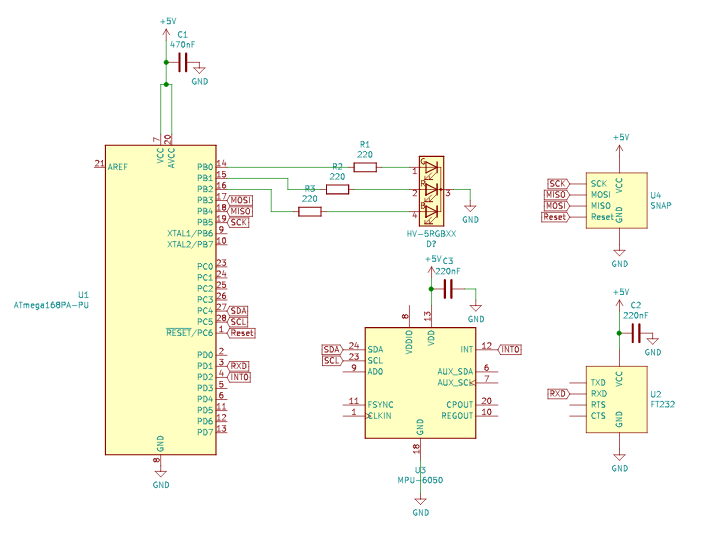
\includegraphics[scale=0.6]{img/schaltplan.png}
                \caption{Schaltplan}
            \end{figure}
            Hierbei ist zu beachten, dass der MPU6050 nicht durch seine Pins im
            Breakboard befestigt wird, sondern waagerecht aufgeklebt wird
            (Siehe \ref{Achsenorentierung}).

        \subsubsection{Kompilieren und Hochladen}
            Sobald die Hardware vollständig aufgebaut wurde, kann der
            \textit{MPLAB SNAP} Programmierer und das \textit{FT232} Modul,
            über Mikro-USB Kabel, an einen Computer angeschlossen werden und die
            \textit{MPLAB IDE} gestartet werden.
            Als nächstes muss das Projekt mit der \textit{MPLAB IDE} geöffnet werden.
            Der Programmer sollte erkannt werden und nach einem Klick auf
            \textit{Run} wird der Code kompiliert und auf die Hardware geladen.
            \\\\
            War dies erfolgreich, kann die Kerze wie im
            Benutzerhandbuch (Siehe \ref{Benutzerhandbuch}) beschrieben, genutzt
            werden.

\section{Problemanalyse}
    \subsection{Betriebsmodi}

        \subsubsection{Laternenmodus}
            Sobald die LED Kerze bewegt wird, wird in den Laternenmodus
            geschaltet werden. Die Kerze leuchtet solange bis keine Bewegung
            mehr detektiert wurde und die Abschaltverzögerung abgelaufen ist.
            Es muss jedoch auch manuell möglich sein, die Kerze abzuschalten.

        \subsubsection{Dekorationsmodus}
            Die Kerze wird manuell in den Dekorationsmodus geschaltet.
            In diesem Modus leuchtet die LED durchgehend bis die
            Abschaltverzögerung die Kerze abschaltet. Wie im
            Laternenmodus soll es möglich sein, die Kerze manuell auszuschalten.


    \subsection{Konfiguration}
        Da die Kerze ausschließlich über Bewegungen konfigurierbar sein soll,
        wird eine Bewegungssteuerung benötigt.
        Dabei wird zwischen Bewegungen entlang einer Achse und Bewegungen
        um eine Achse unterschieden.\\
        Ein Accelerometer kann dabei nur Bewegungen entlang einer Achse,
        wie zum Beispiel das verschieben eines Körpers, messen.
        Dagegen kann ein Gyroskop nur Bewegungen um eine Achse,
        wie zum Beispiel das Rotieren eines Körpers, messen.
        Durch die Kombination der beiden Sensoren erhält man eine
        inertiale Messeinheit und kann somit jede Bewegung eines Körpers
        detektieren. Falls die Startposition sowie Startorientierung bekannt sind,
        kann damit die Position sowie die Orientierung des Körpers im 
        Raum bestimmt werden.
        Somit können Bewegungen durch einen Sensor erkannt werden und als
        Steuerung der Kerze benutzt werden.

    \subsection{Abschaltverzögerung}
        Damit es möglich ist, dass die Kerze sich automatisch nach einer
        konfigurierten Abschaltverzögerung abschaltet, ist es erforderlich,
        dass die vergangene Zeit gemessen werden kann.

    \subsection{Helligkeit und Farbe}
        Über Bewegungssteuerung soll es möglich sein, unter anderem die
        Helligkeit und Farbe einzustellen.
        Dafür wird ein puls-weiten-modulations Verfahren benötigt um die
        einzelnen Farbkanäle der RGB-LED anzusteuern.

    \subsection{Debugging}
        Es muss möglich sein das Programm zu Debuggen. Dazu wird ein Modul
        benötigt, dass Debugausgaben an einem Computer senden kann.

        





\section{Realisation}

  \subsection{Modularisierung}
    Der Programmcode wurde modulweise erstellt, sodass Themengebiete 
    voneinander abgekapselt sind. Durch geschicktes Einbinden kann somit
    Codeverdoppelung vermieden werden.

    \subsubsection{Modulübersicht}

        \paragraph{twi.h}
            Das \textit{Two Wire Interface (TWI)} Modul stellt
            Funktionen zu Verfügung um über ein \textit{TWI}-Bus-System zu 
            kommunizieren. Dabei wurde das Modul sehr \textit{Low-Level}
            gehalten. Das bedeutet unter anderem, dass der Klient dieses Modules 
            selber dafür verantwortlich ist \textit{Start} und \textit{Stop} 
            Konditionen auf den Bus zu setzen. Dabei ist zu beachten, dass dieses
            Modul blockierend arbeitet.

            \begin{figure}[H]
                \centering
                
\includegraphics[scale=0.6]{img/twi.png}
                \caption{twi.h}
            \end{figure}

        \paragraph{led.h}
            Das LED Modul stellt Funktionen rund um die LED Steuerung zu Verfügung.
            Hiermit lässt sich die die LED ein- und ausschalten sowie die Farbe
            konfigurieren und das Blinkverhalten einstellen.

            \begin{figure}[H]
                \centering
                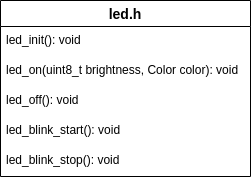
\includegraphics[scale=0.6]{img/led.png}
                \caption{led.h}
            \end{figure}

        \paragraph{timer.h}
            In dem Timer Modul finden sich Funktionen um den Timer zu steuern, der
            die Abschaltverzögerung implementiert.

            \begin{figure}[H]
                \centering
                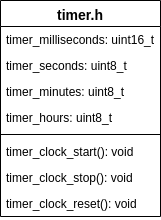
\includegraphics[scale=0.6]{img/timer.png}
                \caption{timer.h}
            \end{figure}

        \paragraph{mpu6050.h}
            Dieses Modul bietet \textit{High-Level} Funktionen um die Daten
            des Accelerometers zu erhalten sowie Konfigurationsmöglichkeiten.
            
            \begin{figure}[H]
                \centering
                
\includegraphics[scale=0.6]{img/mpu.png}
                \caption{mpu6050.h}
            \end{figure}

        \paragraph{config.h}
            Das config Modul bietet Konstanten zur Konfiguration der Kerze.
            So können alle Voreinstellungen bearbeitet werden und an die
            entsprechenden Anforderungen angepasst werden.

        \paragraph{types.h}
            Das types Modul beinhaltet alle Datenstrukturen die für das Programm 
            benötigt werden (Siehe \ref{Datenstrukturen}).

        \paragraph{debug.h}
            Das Debug Modul wird zu debug Zwecken benötigt und implementiert
            somit nur Funktionen um über die \textit{USART} Schnittstelle Daten zu
            senden, jedoch nicht um Daten zu empfangen. Die Daten können dann von einer
            seriellen Schnittstelle an einem Computer betrachtet werden.
            Das Modul arbeitet hierbei blockierend.

            \begin{figure}[H]
                \centering
                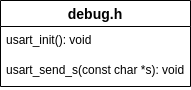
\includegraphics[scale=0.6]{img/debug.png}
                \caption{debug.h}
            \end{figure}
    
    \subsubsection{Programmorganisationsplan}
        \begin{figure}[H]
            \centering
            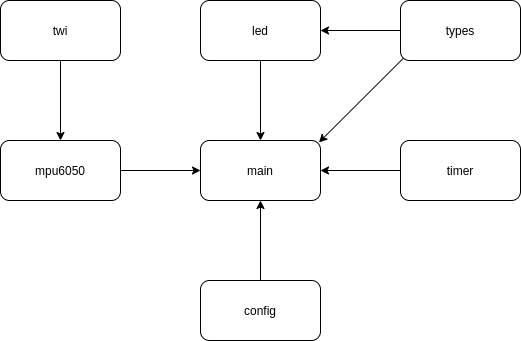
\includegraphics[scale=0.5]{img/pop.png}
            \caption{Programmorganisationsplan}
        \end{figure}


  \newpage
  \subsection{Datenstrukturen}\label{Datenstrukturen}
    Alle Datenstrukturen die für das Programm benötigt werden, befinden sich
    in der \textit{types.h} Datei.

    \subsubsection{State}
        Die \textit{State} Datenstruktur repräsentiert den aktuellen Zustand
        der Zustandsmaschine (Siehe \ref{Zustandsmaschine}).
        \lstinputlisting[caption=State Enum,firstline=11, lastline=21]{../types.h}


    \subsubsection{Delay}
        Die \textit{Delay} Datenstruktur beschreibt die Abschaltverzögerung und
        speichert die Minuten sowie die Stunden nachdem die Kerze sich
        abschalten soll.
        \lstinputlisting[caption=Delay Struct,firstline=23, lastline=29]{../types.h}


    \subsubsection{Color}
        Die \textit{Color} Datenstruktur steht für die LED Farbe und
        speichert die drei Farbkanäle Rot, Grün und Blau. Der Maximalwert
        eines Farbkanals ist 100.
        \lstinputlisting[caption=Color Struct,firstline=31, lastline=38]{../types.h}


    \subsubsection{Config}
        Die \textit{Config} Datenstruktur repräsentiert alle
        Konfigurationsparameter der Kerze und ist aus den anderen oben genannten
        Datenstrukturen kompositioniert.
        Dabei wird zwischen der Laternen- und der Dekorationsabschaltverzögerung
        unterschieden. Zusätzlich hält die Datenstruktur noch die Helligkeit
        deren Maximalwert auch hier 100 beträgt.
        \lstinputlisting[caption=Config Struct,firstline=40, lastline=48]{../types.h}

    
    \subsubsection{setup\_colors}
        Das \textit{setup\_colors} Array speichert die Farbe die die Kerze im
        \textit{SETUP\_DELAY} Zustand annehmen soll.
        \lstinputlisting[caption=setup\_colors Array,firstline=42, lastline=49]{../main.c}

    \subsubsection{lantern\_delays}
        Das \textit{lantern\_delays} Array speichert alle Abschaltverzögerungen für
        den Laternenmodus zwischen denen der Benutzer wählen kann.
        \lstinputlisting[caption=deco\_delays Array,firstline=51, lastline=58]{../main.c}

    \subsubsection{deco\_delays}
        Das \textit{deco\_delays} Array speichert alle Abschaltverzögerungen für
        den Dekorationsmodus zwischen denen der Benutzer wählen kann.
        \lstinputlisting[caption=deco\_delays Array,firstline=60, lastline=67]{../main.c}

    \subsubsection{led\_colors}
        Das \textit{led\_colors} Array speichert alle Farben zwischen denen der
        Benutzer wählen kann.
        \lstinputlisting[caption=led\_colors Array,firstline=69, lastline=76]{../main.c}

  \newpage
  \subsection{Bewegungssteuerung}
  Zum detektieren von Bewegungen wird ein \textit{MPU6050} eingesetzt.
  Dieser Sensor beinhaltet ein drei-Achsen Gyroskop, ein drei-Achsen 
  Accelerometer und ein Temperatursensor.

    \subsubsection{Sensorwahl}
      Da die konstante Erdbeschleunigung von $1g = 9,81\frac{m}{s}$
      die Kerze kontinuierlich in Richtung Erdmittelpunkt beschleunigt,
      reicht das drei-Achsen Accelerometer aus, um die genaue
      Neigung der Kerze zu bestimmen. Zu beachten ist jedoch, dass nur
      Neigungen um die X- und Y-Achsen detektiert werden können.
      Rotationen um die Z-Achse werden von dem Accelerometer nicht
      wahrgenommen da die Z-Achse auf den beiden anderen Achsen steht.
      \\\\
      Alternativ könnte auch das Gyroskop verwendet werden. Darüber lassen
      sich Drehwinkel um die Achsen messen. Da jedoch ein Gyroskop
      $\frac{Winkel}{Zeit}$ als Einheit hat, müsste integriert und die Werte
      aufsummiert werden. Die wahrscheinlichkeit, dass der Sensorwert dabei
      driftet ist sehr hoch und wird somit nicht als Lösung betrachtet.


    \subsubsection{Achsenorentierung}\label{Achsenorentierung}
      Zu beachten ist, dass der Sensor nicht über seine Pins im
      Breakout Board befestigt wird sondern flach auf dem Board
      festgeklebt wird. Daraus ergibt sich folgende Orientierung der
      Achsen.
      \begin{description}       
          \item[Z-Achse] Senkrechte Achse
          \item[Y-Achse] Horizontale Achse
          \item[X-Achse] Senkrecht auf beiden anderen Achsen
      \end{description}



    \subsubsection{Kommunikation}
      Die Sensordaten werden über ein $TWI$ Bus an den Mikrocontroller
      übertragen.

      \paragraph{Senden}
        Als Beispiel eines Sendevorgangs wird die Konfiguration des
        Accelerometers benutzt.
        \lstinputlisting[caption=TWI Sendevorgang,firstline=26, lastline=39]{../mpu6050.c}
        Zunächst wird das Startsignal auf den Bus gelegt und gewartet bis der
        Bus frei ist. Sobald die Kondition eintritt, wird die Schreibadresse des
        \textit{MPU6050} gesetzt. Als nächstes wird die Registeradresse in die
        die Daten geschrieben werden sollen auf den Bus geschrieben und auf das
        \textit{ACK} gewartet. War dies erfolgreich, können die eigentlichen
        Daten auf den Bus geschrieben werden und das Stoppsignal gesendet werden.


      \paragraph{Empfangen}
        Als Beispiel für das Empfangen von Daten wird das auslesen des
        Accelerometers benutzt.
        \lstinputlisting[caption=TWI Empfangsvorgang,firstline=113, lastline=132]{../mpu6050.c}
        Zunächst wird wie beim Senden das Startsignal auf den Bus gelegt,
        die Schreibadresse des \textit{MPU6050} gesetzt und das zu lesenden
        Register gesendet. Nun erfolgt ein wiederholter Start mit der Leseadresse
        des \textit{MPU6050}. Durch \texttt{twi\_read\_ack} wird das erste Byte
        ausgelesen. Der \textit{MPU6050} erhöht nach dem Empfangen des \textit{ACK}
        automatisch die Registeradresse, sodass mit \texttt{twi\_read\_nack}
        das zweite Byte ausgelesen werden kann. Nach dem zweiten Byte wird
        jedoch ein \textit{NACK} gesendet, welches dem \textit{MPU6050} signalisiert,
        dass keine Daten mehr erwartet werden. Nach dem Stoppsignal ist die
        Kommunikation beendet.


    \subsubsection{Kalibrierung}
      Durch die Kalibrierung wird der \textit{null Fehler} kompensiert und damit 
      gewährleistet, dass der Sensor kalibrierte Daten liefert.
      \\
      Ein \textit{null Fehler} entsteht dadurch, dass ein Sensor einen Wert
      liefert der ungleich null ist, obwohl der Sensor sich in Ruhelage
      befindet. Da der Fehler sich selbst bei  baugleichen Sensoren
      unterscheidet, muss für jeden Sensor eine einmalige Kalibrierung erfolgen.
      \\\\
      Über die \texttt{mpu6050\_calibrate} Funktion werden die Werte gemittelt
      und dann über die \texttt{debug\_print} Funktion ausgegeben.
      Dazu wird zunächst der Sensor waagerecht auf eine plane Fläche gelegt,
      sodass die Z-Achse nach oben Zeigt und die Funktion ausgeführt.
      Nun wir der Z-Achsenwert notiert, das Verfahren für alle Achsen
      wiederholt und der entsprechende Achsenwert notiert.
      \\
      Um den eigentlichen Versatz zu berechnen werden folgende Formeln verwendet.
      $$  Versatz_X = 0 - Achsenwert_X $$
      $$  Versatz_Y = 0 - Achsenwert_Y $$
      $$  Versatz_Z = 1 - Achsenwert_Z $$
      Für den benutzen Sensor ergeben sich somit folgende Versätze.
      \begin{center}
        \begin{tabular}{| c | c |}
            \hline
            Achse & Versatz \\
            \hline
            X & $-0.035939$ \\
            \hline
            Y & $0.010786$ \\
            \hline
            Z & $0.187407$ \\
            \hline
        \end{tabular}
      \end{center}
      Der Versatz muss nun auf jeden entsprechenden Wert hinzuaddiert werden um
      den \textit{null Fehler} zu kompensieren.
      \lstinputlisting[caption=Nullfehler Kompension,firstline=136, lastline=138]{../mpu6050.c}


    \subsubsection{Digitale Tiefpassfilterung}
      Um dem Rauschen des Sensors entgegen zu wirken, wird die interne digitale
      Tiefpassfilterung des \textit{MPU6050} benutzt. Dabei wird der Tiefpassfilter
      auf $5Hz$ gestellt um hochfrequentes Rauschen zu filtern.

 



      
  \newpage
  \input{tex/programmierhandbuch/abschaltverzögerung.tex}
  \newpage
  \subsection{LED}
    Als LED kommt eine \textit{HV-5RGBXX} zum Einsatz. Diese wird über drei Pins
    mit jeweiligen 220Ohm Widerstand an den \textit{Atmega168} angeschlossen
    (Siehe \ref{schaltplan}).

\subsubsection{Farbe und Helligkeit}
    Durch die drei Pins die die Grundfarben Rot, Grün und Blau repräsentieren,
    lassen sich über additive Farbmischung unterschiedliche Farben einstellen.
    \\
    Um Intensitäten einstellen zu können wird ein puls-weiten-modulations (PWM)
    Signal pro Pin erzeugt. Hierfür wird der Hardware Timer \textit{TIMER2} des
    \textit{Atmega168} verwendet. Da der Timer jedoch nur zwei Ausgänge bestitz, kann
    kein Hardware PWM Signal, wie zum Beispiel \textit{Fast PWM} verwendet werden,
    sodass ein \textit{Soft-PWM} implementiert wurde.
    
    \lstinputlisting[caption=led\_on,firstline=49, lastline=64]{../led.c}
    Um die LED einzuschalten wird die \texttt{led\_on} Funktion mit den
    jeweiligen Parametern aufgerufen. Zunächst werden die
    Pulsweiten für die einzelnen Farbkanäle berechnet. Diese sagen aus, wie 
    lange der Farbkanal pro Periode eingeschaltet ist. In der Formel wird direkt
    die Helligkeit mit der Farbintensität verrechnet.

    \begin{displaymath}
        Pulsweite = \frac{Helligkeit \cdot Farbintensität}{Farbintensität_{max} \cdot Periodenschritte_{max}}
    \end{displaymath}
    Des weiteren wird der Timer gestartet, sodass dieser mit einer Frequenz von
    $3906Hz$ bzw. alle $256\mu{s}$ die \textit{ISR} ausführt.
    \newpage
    \lstinputlisting[caption=PWM ISR,firstline=75, lastline=115]{../led.c}
    In dieser \textit{ISR} wird der Zähler \texttt{pwm\_step} pro Aufruf inkrementiert und 
    mit den jeweiligen Pulsweiten der Farbkanäle verglichen.
    Liegt der Zähler unterhalb einer Pulsweite, wird der entsprechende Farbkanal
    eingeschaltet. Umgekehrt wird der Farbkanal ausgeschaltet sobald der Zähler
    oberhalb der Pulsweite liegt. Sobald der Zähler die maximalen Periodenschritte
    erreicht hat, wird dieser auf null zurückgesetzt.
    Als maximal Periodenschritte wurde zehn gewählt. Daraus folgt eine Periodendauer
    von ca. 2ms, welches zu schnell für das menschliche Auge ist und somit 
    als kontinuierliches Licht wahrgenommen wird.
    \\\\
    Auch wenn die \textit{TIMER2\_COMPA\_vect\ ISR} nicht rechenintensiv ist, könnte sie verkürzt
    werden, sodass die CPU weniger blockiert. Dazu könnte die Logik in die
    Hauptschleife ausgelagert werden und \texttt{OCR2A} auf die maximale
    Periodenschritte gesetzt werden. Ein vergleich des Periodenschrittes mit
    \texttt{TCNT2} wäre dann äquivalent. Der Vorteil wäre hierbei, dass die
    zeitlich kürzere \textit{ISR} die CPU weniger blockiert.
    Ein jedoch großer Nachteil könnte sein,
    dass die Farben bei hoher CPU Auslastung driften, da nicht genug CPU Zeit
    in der Hauptschleife vorhanden ist um die PWM Signale stabil zu halten.
    \\
    Ein weiterer Ansatz wäre es, zwei hardware Timer zu benutzen und
    \textit{Fast-PWM} einzusetzen. Dabei würde zum Beispiel ein Timer zwei
    Farbkanäle und der andere einen Farbkanal steuern.
    Der Vorteil an dieser Lösung wäre, dass weniger Overhead durch das aufrufen
    der \textit{ISR} auftreten würde. Jedoch werden auch zwei der drei hardware
    Timer des \textit{Atmega168} dafür beansprucht.

\subsubsection{Blinken}
    Um ein Blinken der LED zu realisieren wird der hardware Timer \textit{TIMER1}
    eingesetzt und so konfiguriert, dass seine \textit{TIMER1\_COMPA\_vect ISR}
    ca. mit 4Hz, also vier mal in einer Sekunde blinkt.
    \lstinputlisting[caption=Blink ISR,firstline=42, lastline=47]{../led.c}
    Dabei toggelt die \textit{ISR} das \texttt{led\_blink\_state} Flag und
    manipuliert somit die \\\textit{TIMER2\_COMPA\_vect\ ISR},
    sodass diese die LED komplett ausschaltet wenn das Flag nicht gesetzt ist.
    \lstinputlisting[caption=Blinkbedingung,firstline=82, lastline=85]{../led.c}
    


  \newpage
  \subsection{Stromsparmaßnahmen}
    Da die LED Kerze über einen Akku betrieben werden soll, soll möglichst viel
    Strom gespart werden. Dabei muss abgewogen werden, was wirklich Sinnvoll ist
    und was in Relation zu anderen großen Stromverbrauchern wie der LED nur
    marginale Verbesserungen mit sich bringt.

    \subsubsection{MPU6050}
        Da von dem Sensor nur das Accelerometer verwendet wird, werden das
        Gyroskop sowie der Temperatursensor deaktiviert. Zusätzlich wird die
        Samplerate auf 32Hz runter gesetzt.

    \subsubsection{Atmega168}
        Sobald die LED nicht leuchtet, die Zustandsmaschine sich somit im
        \textit{LED\_OFF} Zustand befindet, wird der Mikrocontroller schlafen
        gelegt. Dabei wird dieser in den \textit{Standbymode} versetzt, sodass
        die Stromaufnahe von ca. $8.5mA$ auf ca. $2.5mA$ des Gesamtsystems zurück
        geht. Dies ist eine Reduktion von $70\%$ und wird die Akkulaufzeit
        verlängern.
        Dies geschieht über den Aufruf der \texttt{sleep} Funktion.

        \lstinputlisting[caption=sleep,firstline=102, lastline=112]{../main.c}
        Dabei werden zunächst alle Interrupts gesperrt, sodass es zu keinen
        \textit{Race Conditions} kommen kann. Ein Beispiel für solch eine
        \textit{Race Condition} wäre, dass die \textit{ISR} die externen
        interrupts deaktiviert, die CPU sich aber im nächsten Moment schlafen legt
        und somit nicht wieder aufwachen kann.\\
        Als nächstes wird das externe Interrupt maskiert, sodass der
        Mikrocontroller nur aufwacht, sobald am \textit{INT0} Pin eine
        steigende Flanke anliegt.
        Durch das Ausführen der \texttt{sei} Funktion werden alle Interrupts wieder aktiviert.
        Zusätzlich wird der nächste Funktionsaufruf unterbrechungsfrei garantiert.
        Somit kann es zu keinen \textit{Race Conditions} mehr kommen und der
        Mikrocontroller kann durch \texttt{sleep\_cpu} schlafen gelegt werden.

        \lstinputlisting[caption=Aufwach ISR,firstline=130, lastline=136]{../main.c}
        Der \textit{Standbymode} wurde dabei ausgewählt, da aus diesem
        der Mikrocontroller in nur sechs Taktzyklen wieder aufwachen kann.
        Das Aufwachen passiert dabei über das \textit{INT0} Interrupt welches
        durch den \textit{MPU6050} ausgelöst wird sobald diesem neue Daten zu
        Verfügung stehen.
        Nach dem Aufwachen wird der Code nach \texttt{sleep\_disbale}
        weiter ausgeführt.


  \subsection{Hauptschleife}
    Die Hauptschleife ist der Kern des Programmes und verwaltet alle Variablen.

    \subsubsection{Zustandsmaschine}\label{Zustandsmaschine}
        Um die verschiedenen Zustände der Kerze zu verwalten, wird eine 
        Zustandsmaschine verwendet. Diese beinhaltet folgende Zustände,
        wobei die Kerze im \textit{LED\_OFF} Zustand startet.
        Bei jedem Zustandswechsel wird das \texttt{lock} Flag aktiviert und
        blockiert solange die Zustandsmaschine bis die Kerze ihre
        Ausgangsposition wieder eingenommen hat. Somit wird verhindert,
        dass eine Bewegung der Kerze mehrere Zustände überspringt.
        Die eigentliche Zustandsmaschine besteht aus dem \texttt{State} Enum
        sowie der \textit{Switch-Anweisung} in der Hauptschleife.

        \begin{figure}[H]
            \centering
            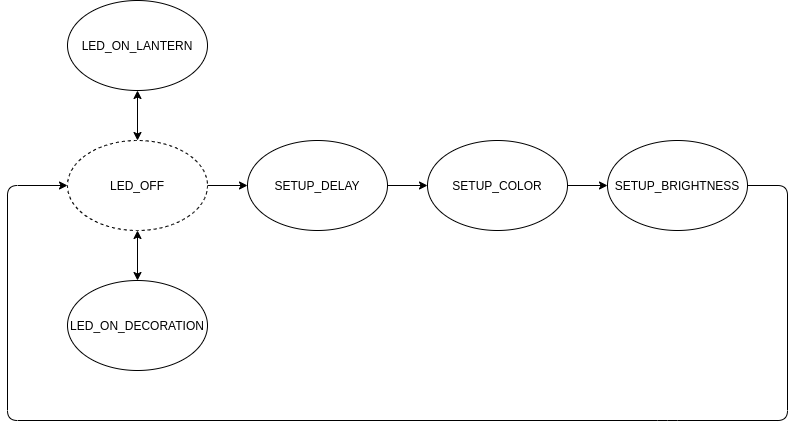
\includegraphics[scale=0.5]{img/state.png}
            \caption{Zustandsmaschine}
        \end{figure}
    
    \subsubsection{Konfiguration}
        In jedem \textit{Setup} Zustand kann das entsprechende Array
        (Siehe \ref{Datenstrukturen}) durchlaufen werden und somit die
        vordefinierten Werte in der \texttt{Config} Datenstruktur gespeichert
        werden. Der einsatz eines Arrays spart in diesem Fall mehrere Zustände,
        da nicht für jeden vordefinierten Wert ein neuer Zustand erstellt werden
        muss. Der Nachteil dieser Lösung ist der höhere Ramverbrauch durch die
        Arrays, welcher jedoch bei einer Arraygröße von drei unerheblich ist.
        Beispielhaft für dieses Verfahren wird der \textit{SETUP\_COLOR} Zustand
        beschrieben.
        \lstinputlisting[caption=SETUP\_COLOR Zustand,firstline=246, lastline=267]{../main.c}
        Die \texttt{setup\_index} Variable wird bei jedem Zustandswechsel auf
        \texttt{SETUP\_DEFAULT\_INDEX}, welches eins ist, gesetzt. Somit
        startet jeder \textit{Setup} Zustand in der Mitte des Arrays und
        ermöglicht es, durch inkrementieren von \texttt{setup\_index} einen
        höheren Wert, sowie durch das dekrementieren der Variable einen
        niedrigeren Wert zu wählen. Dabei muss zusätzlich darauf geachtet werden,
        dass es zu keinem Über- bzw. Unterlauf kommt.



  \newpage
  \subsection{Debug}
    Um das Programm zu debuggen wurde ein eigenes Modul entworfen, welches
    über die \textit{USART} Schnittstelle des \textit{Atmega168} mit einem
    Computer kommunizieren kann. Damit die Debugausgaben nicht händisch
    ein- bzw. auskommentiert werden müssen, wurde ein Makro erstellt welches 
    über das präprozessor Flag \texttt{DEBUG} aktiviert bzw. deaktiviert wird.
    Dabei kann das Flag modulweise aktiviert werden und damit nur einzelne
    Module in den Debugmodus versetzt werden. Sollte das \texttt{DEBUG} Flag
    nicht gesetzt sein, optimiert der Kompilierer den Programmcode raus, sodass
    keine Performance- sowie Platzeinbußen hingenommen werden müssen.
    \lstinputlisting[caption=Debug Makro,firstline=30, lastline=38]{../debug.h}
  \subsection{Voreinstellungen}\label{config}
    Alle voreingestellten Werte, wie zum Beispiel die Farben der Kerze,
    werden in dem \textit{config.h} Modul gehalten. Somit können alle Werte an
    einem Ort eingesehen und gegebenenfalls geändert werden.
    \lstinputlisting[caption=Ausschnitt aus config.h,firstline=42, lastline=55]{../config.h}

  \subsection{Erweiterbarkeit}
    Um das Programm mit neunen Werten zu erweitern, müssen zunächst neue
    Konstanten in der \textit{config.h} definiert werden (Siehe \ref{config}).
    Dann muss das Array was die Voreinstellungen hält mit den neuen Werten
    erweitert werden (Siehe \ref{Datenstrukturen}). 
    Zusätzich muss die \texttt{SETUP\_MAX\_INDEX} Konstante um die Anzahl an
    hinzugefügten Werten addiert werden. Hierbei ist jedoch zu erwähnen, dass
    diese Konstante von allen Arrays verwendet wird.
    Somit müssen alle Arrays um Werte erweitert werden.
    Eine zu empfehlende Verbesserung wäre es, für jedes Array eine eigene
    Konstante anzulegen.


  

  


  
        
        




\section{Programmtests}
    Aufgrund der niedrigen Komplexität des Programmes wurden keine automatischen
    Tests geschrieben. Die Tests wurden daher \textit{per Hand} ausgeführt.
    Dabei wurden alle Funktionen sowohl einzeln als auch im Gesamten getestet 
    und die Ergebnisse über die Debugausgabe überprüft. Zusätzlich wurde 
    die Kerze von Dritten getestet um Betriebsblindheit auszuschließen.

    \subsection{Durchgeführte Tests}
        Alle ausgeführten Tests wurden mit einer zurückgesetzten Kerze getestet,
        sodass sich die Tests gegenseiten nicht beeinflussen.

        \begin{center}
            \begin{longtable}{| p{0.4\textwidth} | p{0.3\textwidth} | p{0.3\textwidth} |}
                \hline
                Testfall & Erwartetes Ergebnis & Erzieltes Ergebnis \\
                \hline

                Starten des Laternenmodus durch Schütteln der Kerze. &
                Die Kerze sollte in der Standardfarbe (Orange), Standardhelligkeit (50\%) leuchten
                und nach der Standardabschaltverzögerung (1 min) abschalten. &
                Die Kerze leuchtet mit ihren Standartwerten und schaltet sich
                nach der Standardabschaltverzögerung ab. \\
                \hline

                Starten des Dekorationsmodus durch nach hinten Kippen der Kerze.&
                Die Kerze sollte in der Standardfarbe (Orange), Standardhelligkeit (50\%) leuchten
                und nach der Standardabschaltverzögerung (30 min) abschalten. &
                Die Kerze leuchtet mit ihren Standartwerten und schaltet sich
                nach der Standardabschaltverzögerung ab. \\
                \hline

                Zurücksetzen der Abschaltverzögerung durch Bewegung im Laternenmodus.
                Dafür wird die Kerze in Laternenmodus versetzt und nach 30 Sekunden
                geschüttelt. &
                Die Kerze sollte nach insgesamt einer Minute und 30 Sekunden nach Testbeginn
                sich ausschalten. &
                Die Kerze schaltet sich nach 1 Minute und 30 Sekunden aus.\\
                \hline

                Ausschalten der Kerze im Laternenmodus. Dafür wird die Kerze
                in den Laternenmodus versetzt und anschließend auf dem Kopf gedreht.&
                Die Kerze sollte sich ausschalten.&
                Die Kerze schaltet sich aus.\\
                \hline

                Ausschalten der Kerze im Dekorationsmodus. Dafür wird die Kerze
                in den Dekorationsmodus versetzt und anschließend auf dem Kopf gedreht.&
                Die Kerze sollte sich ausschalten.&
                Die Kerze schaltet sich aus.\\
                \hline

                Folgende Parameter werden durch den Konfigurationsmodus gesetzt.
                \begin{itemize}
                    \item Abschaltverzögerung: 3 min
                    \item Farbe: Pink
                    \item Helligkeit: 100\%
                \end{itemize}&
                Die Kerze soll in den konfigurierten Parametern leuchten und nach
                der konfigurierten Abschaltverzögerung sich abschalten.&
                Die Kerze leuchtet mit den konfigurierten Parametern und
                schaltet sich nach der konfigurierten Abschaltverzögerung ab.\\
                \hline

                Kombination der Tests. Die Tests werden ohne Zurücksetze
                hintereinander ausgeführt.&
                Die Kerze soll sich in den Tests konsistent und deterministisch verhalten&
                Die Kerze verhält sich in den Tests konsistent und deterministisch\\
                \hline

            \end{longtable}
        \end{center}
  \newpage
  \listoffigures
  \lstlistoflistings
\end{document}